%% abtex2-modelo-trabalho-academico.tex, v-1.9.2 laurocesar
%% Copyright 2012-2014 by abnTeX2 group at http://abntex2.googlecode.com/ 
%%
%% This work may be distributed and/or modified under the
%% conditions of the LaTeX Project Public License, either version 1.3
%% of this license or (at your option) any later version.
%% The latest version of this license is in
%%   http://www.latex-project.org/lppl.txt
%% and version 1.3 or later is part of all distributions of LaTeX
%% version 2005/12/01 or later.
%%
%% This work has the LPPL maintenance status `maintained'.
%% 
%% The Current Maintainer of this work is the abnTeX2 team, led
%% by Lauro César Araujo. Further information are available on 
%% http://abntex2.googlecode.com/
%%
%% This work consists of the files abntex2-modelo-trabalho-academico.tex,
%% abntex2-modelo-include-comandos and abntex2-modelo-references.bib
%%

% ------------------------------------------------------------------------
% ------------------------------------------------------------------------
% abnTeX2: Modelo de Trabalho Academico (tese de doutorado, dissertacao de
% mestrado e trabalhos monograficos em geral) em conformidade com 
% ABNT NBR 14724:2011: Informacao e documentacao - Trabalhos academicos -
% Apresentacao
% ------------------------------------------------------------------------
% ------------------------------------------------------------------------

%-------------------------------------------------------------------------
% Modelo adaptado especificamente para o contexto do PPgSI-EACH-USP por 
% Marcelo Fantinato, com auxílio dos Professores Norton T. Roman, Helton
% H. Bíscaro, e Sarajane M. Peres, em 2015, com muitos agradecimentos aos 
% criadores da classe e do modelo base.
%-------------------------------------------------------------------------

\documentclass[
	% -- opções da classe memoir --
	12pt,				% tamanho da fonte
	% openright,			% capítulos começam em pág ímpar (insere página vazia caso preciso)
	oneside,			% para impressão apenas no anverso (apenas frente). Oposto a twoside
	a4paper,			% tamanho do papel. 
	% -- opções da classe abntex2 --
	%chapter=TITLE,		% títulos de capítulos convertidos em letras maiúsculas
	%section=TITLE,		% títulos de seções convertidos em letras maiúsculas
	%subsection=TITLE,	% títulos de subseções convertidos em letras maiúsculas
	%subsubsection=TITLE,% títulos de subsubseções convertidos em letras maiúsculas
	% -- opções do pacote babel --
	english,			% idioma adicional para hifenização
	%french,				% idioma adicional para hifenização
	%spanish,			% idioma adicional para hifenização
	brazil				% o último idioma é o principal do documento
	]{abntex2ppgsi}
% * <gustavodm.ramos@gmail.com> 2016-12-04T17:24:21.541Z:
%
% ^.
% ---
% Pacotes básicos 
% ---
% \usepackage{lmodern}			% Usa a fonte Latin Modern			
% \usepackage[T1]{fontenc}		% Selecao de codigos de fonte.
\usepackage[utf8]{inputenc}		% Codificacao do documento (conversão automática dos acentos)
\usepackage{lastpage}			% Usado pela Ficha catalográfica
\usepackage{indentfirst}		% Indenta o primeiro parágrafo de cada seção.
\usepackage{color}				% Controle das cores
\usepackage{graphicx}			% Inclusão de gráficos
\usepackage{microtype} 			% para melhorias de justificação
\usepackage{pdfpages}     %para incluir pdf
\usepackage{algorithm}			%para ilustrações do tipo algoritmo
\usepackage{mdwlist}			%para itens com espaço padrão da abnt
\usepackage[noend]{algpseudocode}			%para ilustrações do tipo algoritmo
\usepackage[T1]{fontenc}
% ---
% Pacotes adicionais, usados apenas no âmbito do Modelo Canônico do abnteX2
% ---
\usepackage{lipsum}				% para geração de dummy text
% ---

% ---
% Pacotes de citações
% ---
\usepackage[brazilian,hyperpageref]{backref}	 % Paginas com as citações na bibl
\usepackage[alf]{abntex2cite}	% Citações padrão ABNT

% --- 
% CONFIGURAÇÕES DE PACOTES
% --- 

% ---
% Configurações do pacote backref
% Usado sem a opção hyperpageref de backref
\renewcommand{\backrefpagesname}{Citado na(s) página(s):~}
% Texto padrão antes do número das páginas
\renewcommand{\backref}{}
% Define os textos da citação
\renewcommand*{\backrefalt}[4]{
	\ifcase #1 %
		Nenhuma citação no texto.%
	\or
		Citado na página #2.%
	\else
		Citado #1 vezes nas páginas #2.%
	\fi}%
% ---

% ---
% Informações de dados para CAPA e FOLHA DE ROSTO
% ---

%-------------------------------------------------------------------------
% Comentário adicional do PPgSI - Informações sobre o ``título'':
%
% Em maiúscula apenas a primeira letra da sentença (do título), exceto 
% nomes próprios, geográficos, institucionais ou Programas ou Projetos ou 
% siglas, os quais podem ter letras em maiúscula também.
%
% O subtítulo do trabalho é opcional.
% Sem ponto final.
%
% Atenção: o título da Dissertação na versão corrigida não pode mudar. 
% Ele deve ser idêntico ao da versão original.
%
%-------------------------------------------------------------------------
\titulo{Seleção entre estratégias de geração automática de dados de teste por meio de métricas estáticas de softwares orientados a objetos}

%-------------------------------------------------------------------------
% Comentário adicional do PPgSI - Informações sobre o ``autor'':
%
% Todas as letras em maiúsculas.
% Nome completo.
% Sem ponto final.
%-------------------------------------------------------------------------
\autor{\uppercase{GUSTAVO DA MOTA RAMOS}}

%-------------------------------------------------------------------------
% Comentário adicional do PPgSI - Informações sobre o ``local'':
%
% Não incluir o ``estado''.
% Sem ponto final.
%-------------------------------------------------------------------------
\local{São Paulo}

%-------------------------------------------------------------------------
% Comentário adicional do PPgSI - Informações sobre a ``data'':
%
% Colocar o ano do depósito (ou seja, o ano da entrega) da respectiva 
% versão, seja ela a versão original (para a defesa) seja ela a versão 
% corrigida (depois da aprovação na defesa). 
%
% Atenção: Se a versão original for depositada no final do ano e a versão 
% corrigida for entregue no ano seguinte, o ano precisa ser atualizado no 
% caso da versão corrigida. 
% Cuidado, pois o ano da ``capa externa'' também precisa ser atualizado 
% nesse caso.
%
% Não incluir o dia, nem o mês.
% Sem ponto final.
%-------------------------------------------------------------------------
\data{2018}

%-------------------------------------------------------------------------
% Comentário adicional do PPgSI - Informações sobre o ``Orientador'':
%
% Se for uma professora, trocar por ``Profa. Dra.''
% Nome completo.
% Sem ponto final.
%-------------------------------------------------------------------------
\orientador{Prof. Dr. Marcelo Medeiros Eler}

%-------------------------------------------------------------------------
% Comentário adicional do PPgSI - Informações sobre o ``Coorientador'':
%
% Opcional. Incluir apenas se houver co-orientador formal, de acordo com o 
% Regulamento do Programa.
%
% Se for uma professora, trocar por ``Profa. Dra.''
% Nome completo.
% Sem ponto final.
%-------------------------------------------------------------------------
%\coorientador{Prof. Dr. Fulano de Tal}

\tipotrabalho{Dissertação (Mestrado)}

\preambulo{
%-------------------------------------------------------------------------
% Comentário adicional do PPgSI - Informações sobre o texto ``Versão 
% original'':
%
% Não usar para Qualificação.
% Não usar para versão corrigida de Dissertação.
%
%-------------------------------------------------------------------------
Versão original
%-------------------------------------------------------------------------
% Comentário adicional do PPgSI - Informações sobre o ``texto principal do
% preambulo'':
%
% Para Qualificação, trocar por: Texto de Exame de Qualificação apresentado à Escola de Artes, Ciências e Humanidades da Universidade de São Paulo como parte dos requisitos para obtenção do título de Mestre em Ciências pelo Programa de Pós-graduação em Sistemas de Informação.
%
%-------------------------------------------------------------------------
\newline \newline \newline Dissertação apresentada à Escola de Artes, Ciências e Humanidades da Universidade de São Paulo para obtenção do título de Mestre em Ciências pelo Programa de Pós-graduação em Sistemas de Informação. 
%
\newline \newline Área de concentração: Metodologia e Técnicas da Computação
%-------------------------------------------------------------------------
% Comentário adicional do PPgSI - Informações sobre o texto da ``Versão 
% corrigida'':
%
% Não usar para Qualificação.
% Não usar para versão original de Dissertação.
% 
% Substituir ``xx de xxxxxxxxxxxxxxx de xxxx'' pela ``data da defesa''.
%
%-------------------------------------------------------------------------
\newline \newline \newline Versão corrigida contendo as alterações solicitadas pela comissão julgadora em xx de xxxxxxxxxxxxxxx de xxxx. A versão original encontra-se em acervo reservado na Biblioteca da EACH-USP e na Biblioteca Digital de Teses e Dissertações da USP (BDTD), de acordo com a Resolução CoPGr 6018, de 13 de outubro de 2011.}
% ---


% ---
% Configurações de aparência do PDF final

% alterando o aspecto da cor azul
\definecolor{blue}{RGB}{41,5,195}

% informações do PDF
\makeatletter
\hypersetup{
     	%pagebackref=true,
		pdftitle={\@title}, 
		pdfauthor={\@author},
    	pdfsubject={\imprimirpreambulo},
	    pdfcreator={LaTeX com abnTeX2 adaptado para o PPgSI-EACH-USP},
		pdfkeywords={abnt}{latex}{abntex}{abntex2}{qualificação de mestrado}{dissertação de mestrado}{ppgsi}, 
		colorlinks=true,       		% false: boxed links; true: colored links
    	linkcolor=blue,          	% color of internal links
    	citecolor=blue,        		% color of links to bibliography
    	filecolor=magenta,      		% color of file links
		urlcolor=blue,
		bookmarksdepth=4
}
\makeatother
% --- 

% --- 
% Espaçamentos entre linhas e parágrafos 
% --- 

% O tamanho do parágrafo é dado por:
\setlength{\parindent}{1.25cm}

% Controle do espaçamento entre um parágrafo e outro:
\setlength{\parskip}{0cm}  % tente também \onelineskip
\renewcommand{\baselinestretch}{1.5}

% ---
% compila o indice
% ---
\makeindex
% ---

	% Controlar linhas orfas e viuvas
  \clubpenalty10000
  \widowpenalty10000
  \displaywidowpenalty10000

% ----
% Início do documento
% ----
\begin{document}

% Retira espaço extra obsoleto entre as frases.
\frenchspacing 

% ----------------------------------------------------------
% ELEMENTOS PRÉ-TEXTUAIS
% ----------------------------------------------------------
% \pretextual

% ---
% Capa
% ---
%-------------------------------------------------------------------------
% Comentário adicional do PPgSI - Informações sobre a ``capa'':
%
% Esta é a ``capa'' principal/oficial do trabalho, a ser impressa apenas 
% para os casos de encadernação simples (ou seja, em ``espiral'' com 
% plástico na frente).
% 
% Não imprimir esta ``capa'' quando houver ``capa dura'' ou ``capa brochura'' 
% em que estas mesmas informações já estão presentes nela.
%
%-------------------------------------------------------------------------
\imprimircapa
% ---

% ---
% Folha de rosto
% (o * indica que haverá a ficha bibliográfica)
% ---
\imprimirfolhaderosto*
% ---

% ---
% Inserir a autorização para reprodução e ficha bibliografica
% ---

%-------------------------------------------------------------------------
% Comentário adicional do PPgSI - Informações sobre o texto da 
% ``autorização para reprodução e ficha bibliografica'':
%
% Página a ser usada apenas para Dissertação (tanto na versão original 
% quanto na versão corrigida).
%
% Solicitar a ficha catalográfica na Biblioteca da EACH. 
% Duas versões devem ser solicitadas, em dois momentos distintos: uma vez 
% para a versão original, e depois outra atualizada para a versão 
% corrigida.
%
% Atenção: esta página de ``autorização para reprodução e ficha 
% catalográfica'' deve ser impressa obrigatoriamente no verso da folha de 
% rosto.
%
% Não usar esta página para Qualificação.
%
% Substitua o arquivo ``fig_ficha_catalografica.pdf'' abaixo referenciado 
% pelo PDF elaborado pela Biblioteca
%
%-------------------------------------------------------------------------
\begin{fichacatalografica}
    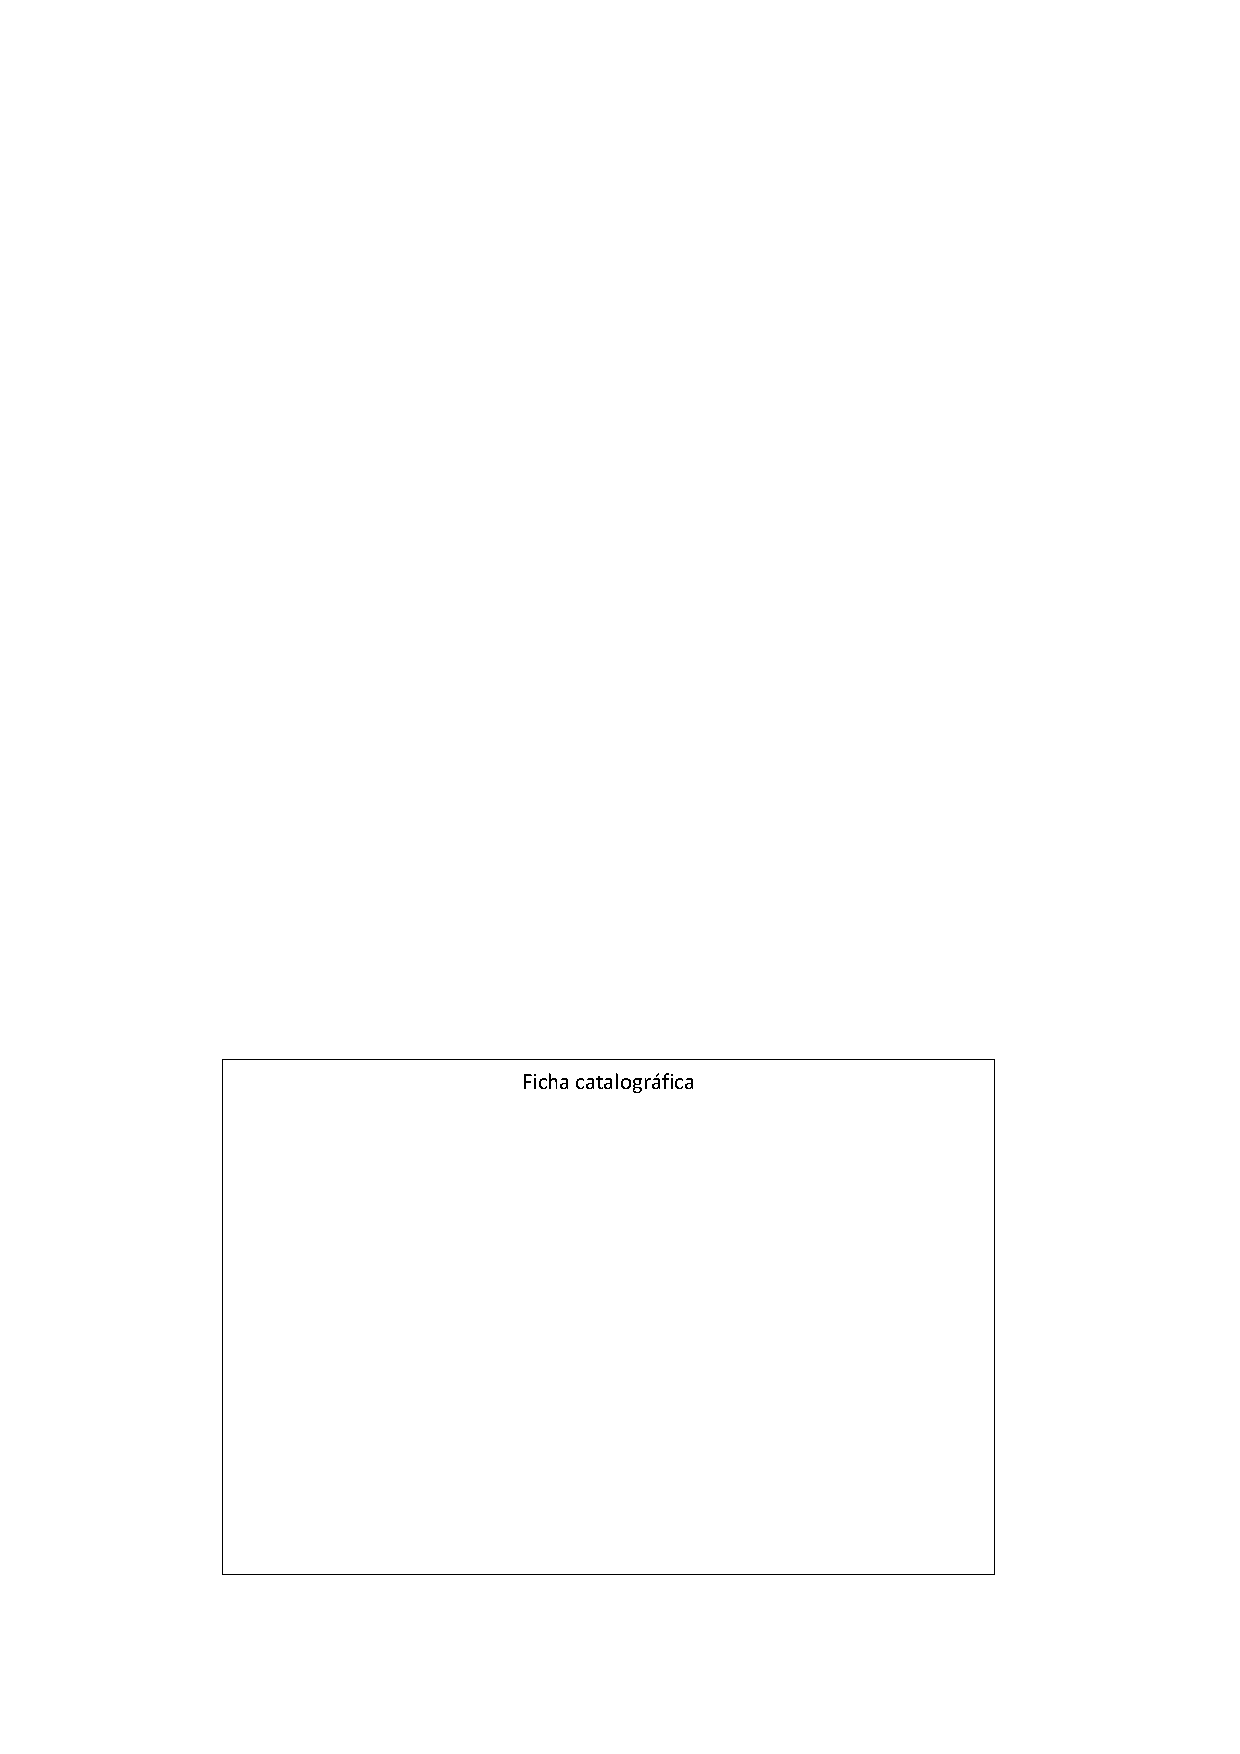
\includepdf{fig_ficha_catalografica.pdf}
\end{fichacatalografica}

% ---
% Inserir errata
% ---
%-------------------------------------------------------------------------
% Comentário adicional do PPgSI - Informações sobre ``Errata'':
%
% Usar esta página de errata apenas em casos de excepcionais, e apenas 
% para a versão corrigida da Dissertação. Por exemplo, quando depois de
% já depositada e publicada a versão corrigida, ainda assim verifica-se
% a necessidade de alguma correção adicional.
%
% Se precisar usar esta página, busque a forma correta (o modelo correto) 
% para fazê-lo, de acordo com a norma ABNT.
%
% Não usar esta página para versão original de Dissertação.
% Não usar esta página para Qualificação.
%
%-------------------------------------------------------------------------
\begin{errata}
Elemento opcional para versão corrigida, depois de depositada.
\end{errata}
% ---

% ---
% Inserir folha de aprovação
% ---

\begin{folhadeaprovacao}
%-------------------------------------------------------------------------
% Comentário adicional do PPgSI - Informações sobre ``Folha da aprovação'':
%
% Para Qualificação, trocar por: Texto de Exame de Qualificação de autoria de Fulano de Tal, sob o título \textbf{``\imprimirtitulo''}, apresentado à Escola de Artes, Ciências e Humanidades da Universidade de São Paulo, como parte dos requisitos para obtenção do título de Mestre em Ciências pelo Programa de Pós-graduação em Sistemas de Informação, na área de concentração Metodologia e Técnicas da Computação, aprovado em \_\_\_ de \_\_\_\_\_\_\_\_\_\_\_\_\_\_ de \_\_\_\_\_\_ pela comissão examinadora constituída pelos doutores:
%
% Substituir ``Fulano de Tal'' pelo nome completo do autor do trabalho, com 
% apenas as iniciais em maiúsculo.
%
% Substiuir ``___ de ______________ de ______'' por: 
%     - Para versão original de Dissertação: deixar em branco, pois a data 
%       pode mudar, mesmo que ela já esteja prevista.
%     - Para versão corrigida de Dissertação: usar a data em que a defesa 
%       efetivamente ocorreu.
%
%-------------------------------------------------------------------------
\noindent Dissertação de autoria de Fulano de Tal, sob o título \textbf{``\imprimirtitulo''}, apresentada à Escola de Artes, Ciências e Humanidades da Universidade de São Paulo, para obtenção do título de Mestre em Ciências pelo Programa de Pós-graduação em Sistemas de Informação, na área de concentração Metodologia e Técnicas da Computação, aprovada em \_\_\_\_\_\_\_ de \_\_\_\_\_\_\_\_\_\_\_\_\_\_\_\_\_\_\_\_\_\_ de \_\_\_\_\_\_\_\_\_\_ pela comissão julgadora constituída pelos doutores:

\vspace*{3cm}

\begin{center}
%-------------------------------------------------------------------------
% Comentário adicional do PPgSI - Informações sobre ``assinaturas'':
%
% Para Qualificação e para versão original de Dissertação: deixar em 
% branco (ou seja, assim como está abaixo), pois os membros da banca podem
% mudar, mesmo que eles já estejam previstos.
% 
% Para versão corrigida de Dissertação: usar os dados dos examinadores que 
% efetivamente participaram da defesa. 
% 
% Em nenhum caso há realmente necessidade de assinaturas.
%
% Para versão corrigida de Dissertação: em caso de ``professora'', trocar 
% por ``Profa. Dra.'' 
% 
% Para versão corrigida de Dissertação: ao colocar os nomes dos 
% examinadores, remover o sublinhado
% 
% Para versão corrigida de Dissertação: ao colocar os nomes dos 
% examinadores, usar seus nomes completos, exatamente conforme constam em 
% seus Currículos Lattes
% 
% Para versão corrigida de Dissertação: ao colocar os nomes das 
% instituições, remover o sublinhado e remover a palavra ``Instituição:''
%
% Não abreviar os nomes das instituições.
%
%-------------------------------------------------------------------------
\textbf{Prof. Dr. \_\_\_\_\_\_\_\_\_\_\_\_\_\_\_\_\_\_\_\_\_\_\_\_\_\_\_\_\_\_\_\_\_\_\_\_\_\_\_\_\_\_\_\_\_\_\_\_\_\_\_\_\_\_\_\_\_\_} 
\\ Presidente 
\\ \vspace*{0.1cm} 
Instituição: \_\_\_\_\_\_\_\_\_\_\_\_\_\_\_\_\_\_\_\_\_\_\_\_\_\_\_\_\_\_\_\_\_\_\_\_\_\_\_\_\_\_\_\_\_\_\_\_\_\_\_\_\_\_\_\_\_\_ 

\vspace*{2cm}

\textbf{Prof. Dr. \_\_\_\_\_\_\_\_\_\_\_\_\_\_\_\_\_\_\_\_\_\_\_\_\_\_\_\_\_\_\_\_\_\_\_\_\_\_\_\_\_\_\_\_\_\_\_\_\_\_\_\_\_\_\_} 
\\ \vspace*{0.2cm} 
Instituição: \_\_\_\_\_\_\_\_\_\_\_\_\_\_\_\_\_\_\_\_\_\_\_\_\_\_\_\_\_\_\_\_\_\_\_\_\_\_\_\_\_\_\_\_\_\_\_\_\_\_\_\_\_\_\_\_

\vspace*{2cm}

\textbf{Prof. Dr. \_\_\_\_\_\_\_\_\_\_\_\_\_\_\_\_\_\_\_\_\_\_\_\_\_\_\_\_\_\_\_\_\_\_\_\_\_\_\_\_\_\_\_\_\_\_\_\_\_\_\_\_\_\_\_} 
\\ \vspace*{0.2cm} 
Instituição: \_\_\_\_\_\_\_\_\_\_\_\_\_\_\_\_\_\_\_\_\_\_\_\_\_\_\_\_\_\_\_\_\_\_\_\_\_\_\_\_\_\_\_\_\_\_\_\_\_\_\_\_\_\_\_\_

\vspace*{2cm}

\textbf{Prof. Dr. \_\_\_\_\_\_\_\_\_\_\_\_\_\_\_\_\_\_\_\_\_\_\_\_\_\_\_\_\_\_\_\_\_\_\_\_\_\_\_\_\_\_\_\_\_\_\_\_\_\_\_\_\_\_\_} 
\\ \vspace*{0.2cm} 
Instituição: \_\_\_\_\_\_\_\_\_\_\_\_\_\_\_\_\_\_\_\_\_\_\_\_\_\_\_\_\_\_\_\_\_\_\_\_\_\_\_\_\_\_\_\_\_\_\_\_\_\_\_\_\_\_\_\_

\end{center}
  
\end{folhadeaprovacao}
% ---

% ---
% Dedicatória
% ---
%-------------------------------------------------------------------------
% Comentário adicional do PPgSI - Informações sobre ``Dedicatória'': 
%
% Opcional para Dissertação.
% Não sugerido para Qualificação.
% 
%-------------------------------------------------------------------------

% ---

% ---
% Agradecimentos
% ---
%-------------------------------------------------------------------------
% Comentário adicional do PPgSI - Informações sobre ``Agradecimentos'': 
%
% Opcional para Dissertação.
% Não sugerido para Qualificação.
% 
% Lembrar de agradecer agências de fomento e outras instituições similares.
%
%-------------------------------------------------------------------------

% ---

% ---
% Epígrafe
% ---
%-------------------------------------------------------------------------
% Comentário adicional do PPgSI - Informações sobre ``Epígrafe'': 
%
% Opcional para Dissertação.
% Não sugerido para Qualificação.
% 
%-------------------------------------------------------------------------

% ---

% ---
% RESUMOS
% ---



% resumo em inglês
%-------------------------------------------------------------------------
% Comentário adicional do PPgSI - Informações sobre ``resumo em inglês''
% 
% Caso a Qualificação ou a Dissertação inteira seja elaborada no idioma inglês, 
% então o ``Abstract'' vem antes do ``Resumo''.
% 
%-------------------------------------------------------------------------


% ---
% ---
% inserir lista de figuras
% ---
\pdfbookmark[0]{\listfigurename}{lof}
\listoffigures*
\cleardoublepage
% ---

% ---
% inserir lista de algoritmos
% ---
\pdfbookmark[0]{\listalgorithmname}{loa}
\listofalgorithms
\cleardoublepage

% ---
% inserir lista de tabelas
% ---
\pdfbookmark[0]{\listtablename}{lot}
\listoftables*
\cleardoublepage
% ---

% ---
% inserir lista de abreviaturas e siglas
% ---
%-------------------------------------------------------------------------
% Comentário adicional do PPgSI - Informações sobre ``Lista de abreviaturas 
% e siglas'': 
%
% Opcional.
% Uma vez que se deseja usar, é necessário manter padrão e consistência no
% trabalho inteiro.
% Se usar: inserir em ordem alfabética.
%
%-------------------------------------------------------------------------

% ---

% ---
% inserir lista de símbolos
% ---
%-------------------------------------------------------------------------
% Comentário adicional do PPgSI - Informações sobre ``Lista de símbolos'': 
%
% Opcional.
% Uma vez que se deseja usar, é necessário manter padrão e consistência no
% trabalho inteiro.
% Se usar: inserir na ordem em que aparece no texto.
% 
%-------------------------------------------------------------------------

% ---

% ---
% inserir o sumario
% ---
\pdfbookmark[0]{\contentsname}{toc}
\tableofcontents*
\cleardoublepage
% ---



% ----------------------------------------------------------
% ELEMENTOS TEXTUAIS
% ----------------------------------------------------------
\textual



%-------------------------------------------------------------------------
% Comentário adicional do PPgSI - Informações sobre ``títulos de seções''
% 
% Para todos os títulos (seções, subseções, tabelas, ilustrações, etc):
%
% Em maiúscula apenas a primeira letra da sentença (do título), exceto 
% nomes próprios, geográficos, institucionais ou Programas ou Projetos ou
% siglas, os quais podem ter letras em maiúscula também.
%
%-------------------------------------------------------------------------
\chapter{Introdução}
Produtos de software de diferentes tamanhos e complexidades são utilizados todos os dias em atividades profissionais ou de entretenimento. Em qualquer circunstância, entretanto, a falta de qualidade em produtos pode caracterizar uma situação preocupante para seus produtores \cite{hilburn2002software}  \cite{binder1994test}, uma vez que cada vez mais os níveis aceitáveis de qualidade de um software estão aumentando, tanto no que se refere ao seu comportamento observável externamente quanto ao seu processo de desenvolvimento e estrutura interna \cite{linda2006quality} \cite{bashir2008test} \cite{graham2008foundations}.


O teste de software \cite{tahir2014test} é a maneira mais popular de verificar se um software atende às especificações descritas e cumpre o papel desejado pelos interessados \cite{sommerville2008engenharia}. Ela consiste na execução do programa sob teste para revelar seus defeitos. Para isso, casos de teste são gerados de maneira que satisfaçam a diversos critérios, em geral baseados na especificação e na implementação do software \cite{pezze2008software}. 

Entretanto, gerar casos de teste para testar o software nos mais diversos contextos e dados de entrada é uma das atividades mais custosas no ciclo de vida de software, requisitando muito tempo e esforço para o seu planejamento, execução e manutenção. \cite{tahir2014test}. Consequentemente, pesquisadores e profissionais da área passaram então a desenvolver  abordagens para gerar casos de teste automaticamente e assim reduzir o custo e a complexidade desta tarefa. Diversas técnicas já foram utilizadas com teste objetivo: geração de testes randômicos \cite{Pacheco2007}; execução simbólica \cite{Cadar2013}; teste baseado em modelos \cite{dick93}; e teste baseado em buscas \cite{McMinn2004, Harman2012}. Diversas ferramentas já foram desenvolvidas utilizando uma ou mais dessas técnicas, como, por exemplo, Randoop \cite{Pacheco2007}, DART \cite{Godefroid2005}, CUTE \cite{Sen2005}, JCute \cite{Sen2006}, Klee \cite{Cadar2008}, JavaPathFinder \cite{Visser2004}, PEX \cite{Tillmann2008} e EvoSuite \cite{Fraser2011}.

Em particular, a técnica de teste baseado em busca tem sido amplamente utilizada para a geração de casos de teste. Neste contexto, destaca-se a ferramenta EvoSuite que é capaz de gerar conjuntos de casos de teste para programas escritos em Java automaticamente. Ela utiliza um algoritmo genético para selecionar os melhores dados de teste e produzir os conjuntos de casos de teste que atingem altos níveis de cobertura estrutural e escore de mutação \cite{Fraser2011}. Esta ferramenta já foi extensivamente avaliada no que se refere à eficácia e escalabilidade \cite{Fraser2013, Rojas2017, Fraser2015, Fraser2014}, e recentemente foi a ferramenta que obteve a maior pontuação na competição de ferramentas de geração de teste unitários promovida anualmente pelo Workshop on Search-Based Software Testing \cite{Fraser2017}.

Recentemente, novos algoritmos evolutivos foram adicionados à ferramenta EvoSuite como alternativa ao algoritmo genético padrão para a geração de casos de teste \cite{Campos2017}:  algoritmo genético monotônico, algoritmo genético de regime permanente (do inglês, steady state), 1 + ($\lambda$,$\lambda$), $\mu$ + $\lambda$, MOSA (Many-Objective Sorting Algorithm) e DynaMOSA (dynamic MOSA); além da geração randômica já implementada anteriormente. Um estudo comparativo utilizando 346 classes selecionadas randomicamente de um conjunto de 117 projetos de código aberto mostrou que a escolha do algoritmo utilizado na geração de casos de teste influencia os resultados, e que diferentes configurações podem favorecer diferentes algoritmos.

\section{Problema de pesquisa}

O estudo realizado para comparar a eficácia dos algoritmos na geração de casos de teste implementados na ferramenta EvoSuite mostrou que a escolha do algoritmo importa. Entretanto, nenhuma análise mais criteriosa foi realizada para identificar em que situações ou para que tipo de classe um algoritmo é melhor do que outro. Portanto, as seguintes questões de pesquisa emergem neste contexto:

\begin{itemize}
  \item Quais são as características das classes sob teste que podem influenciar a eficiência e a eficácia dos algoritmos evolutivos utilizados na geração de casos de teste?
  \item Existem padrões de características para os quais um algoritmo específico geralmente vai obter melhor resultado?
\end{itemize}

\section{Objetivos}

Neste contexto, o objetivo geral deste projeto de pesquisa  é definir uma hiper-heurística para escolher o melhor algoritmo evolutivo na geração de casos de teste de acordo com o problema em mãos. Desta forma, ao invés de utilizar um único algoritmo para gerar todos os casos de teste de um projeto, os casos de teste de cada classe podem ser gerados por diferentes algoritmos dependendo das suas características.

Os objetivos específicos deste projeto de pesquisa são os seguintes:

\begin{enumerate}
	\item Mapear sistematicamente as métricas de software mais utilizadas para estimar a testabilidade de um software.
	\item Selecionar métricas de testabilidade que tem maior probabilidade de influenciar os resultados dos algoritmos na geração de casos de teste. Essa seleção será realizada utilizando-se a correlação entre as métricas e os resultados obtidos pelos algoritmos evolutivos em termos de cobertura de código dos casos de teste gerados por eles.
	\item Utilizar um algoritmo de reconhecimento de padrões para analisar as métricas de testabilidade de uma classe e classificá-la de acordo com o algoritmo de geração de testes mais adequado.
	\item Implementar uma hiper-heurística em uma ferramenta de geração de casos de teste para selecionar o melhor algoritmo evolutivo de acordo com a classe a ser testada.
\end{enumerate}

\section{Justificativa}
Os diversos algoritmos e abordagens de geração de casos de teste encontrados no ambiente acadˆemico e industrial possuem pontos fracos e fortes. Em especial, a técnica de teste baseado em busca tem sido amplamente utilizada para gerar casos de teste, e muitos dos alguns dos seus algoritmos conseguem convergir para resultados  ótimos mais rapidamente do que os outros, mas n não conseguem tratar de situações mais complexas, por exemplo. Portanto, utilizar o algoritmo que consegue obter os melhores resultados e convergir mais rapidamente para cada classe do projeto a ser testado irá aumentar consideravelmente a eficiência e a eficácia de ferramentas de geração de casos de teste como a EvoSuite, por exemplo. Além disso, os resultados obtidos podem encorajar a implementaçã de algoritmos evolutivos que são utilizados em outras áreas mas que ainda não utilizados na geração de casos teste.

\section{Método de pesquisa}
Este projeto será, conduzido usando um método indutivo com objetivos de caráter exploratório, descritivo e experimental. Mais detalhes dos materiais e métodos de pesquisa utilizados neste projeto de pesquisa estã apresentados no Capítulo 5.

\section{Organização do documento}
Esta proposta de pequisa está organizada da seguinte forma. No Capítulo 2 são apresentados os conceitos mais importantes que embasam este projeto.

\chapter{Teste de software: Aspectos conceituais e econômicos}
No presente capítulo será apresentado uma síntese dos conceitos base com o objetivo de fundamentação teórica dos capítulos seguintes e auxílio na estrutura do presente documento.

\section{Teste de software}
O teste de software é uma subárea da engenharia de software que compreende as atividades capazes de determinar se um software em análise contém erros \cite{gerhart1975} com objetivo encontrar falhas e não de provar a corretitude de software, estes não são capazes de demonstrar se um software em análise está livre de defeitos ou que irá se comportar como esperado em todas as circunstâncias, ou seja, testes são responsáveis somente por evidenciar a presença de possíveis erros e não a falta destes \cite{pfleeger2010}. A partir destes é possível validar se o software cumpre o propósito de desenvolvimento e por fim eliminar possíveis defeitos e assim garantir maior qualidade de software \cite{Sommerville2010}. 

Para executar testes de software, é necessário simular sua execução e validar, a partir dos resultados extraídos da execução, possíveis anomalias e erros, ou seja, testes de software são executados com dados artificiais \cite{Sommerville2010}.

\begin{figure}[H]% H manda colocar exatamente nessa posição no texto (relativa aos parágrafos anterior e posterior)
	\centering
 	  \caption{Modelo de teste de software}
		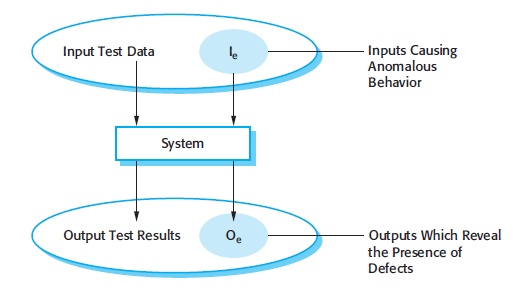
\includegraphics{modelo-teste.png}
	\label{fig:tipos-custo-arvore}
  \source{\cite{Sommerville2010}}
\end{figure}

De acrodo com \cite{pressman2009engenharia} e \cite{Davis1995} são notórios os princípios de teste: 

\begin{enumerate}
\item Todos os testes devem ser rastreáveis aos requisitos de usuários;
\item Testes devem ser planjeados antes de sua execução;
\item O princípio de pareto deve ser aplicado ao teste de software;
\item Testes devem começar as menores unidades afim de atingir partes maiores de software;
\item Testes exaustivos não são possíveis.
\end{enumerate}


\section{Qualidade de software e aspectos econômicos}

A Garantia de Qualidade ou \textit{Quality Assurance} é considerada uma das partes mais caras do desenvolvimento de software \cite{wagner2005}, o conceito de garantia de qualidade tornou-se mais evidente após a primeira conferência de engenharia de software com o propósito de estabelecer melhores princípios e estratégias econômicas para atingir um estado viável de software, esta conferência de em 1968 foi responsável	 inclusive a disciplina de teste e controle de qualidade em diversas  fases de desenvolvimento de software desde então \cite{repasi2009}.

De fato, os custos de garantia de qualidade são elevados \cite{wagner2005} \cite{Korel1990} já que consistem em todo e qualquer valor investido em atividades cujo propósito almeja qualidade de software \cite{pressman2009engenharia}, porém é notável que fatores econômicos em melhoria de qualidade não são bem aceitos por todos os interessados no desenvolvimento de software e que inclusive exista uma certa confusão sobre o valor de negócio da qualidade de desenvolvimento de software \cite{slaughter1998} já que teste de software é uma atividade trabalhosa e cara \cite{Korel1990} mas estes investimentos estes são importantes e devem ser planejados visto que cada valor gasto em horas de trabalho e não investido em retrabalho pode ser usado para melhorias rápidas em produtos e processo existentes \cite{slaughter1998}.

Os custos direcionados à qualidade de software são categorizados em \textit{conformance} e \textit{nonconformance} \cite{ slaughter1998}\cite{pressman2009engenharia} como demonstrado na figura a seguir: 

\begin{figure}[H]% H manda colocar exatamente nessa posição no texto (relativa aos parágrafos anterior e posterior)
	\centering
 	  \caption{Hierarquia da classificação dos tipos de custo presentes em desenvolvimento de software}
		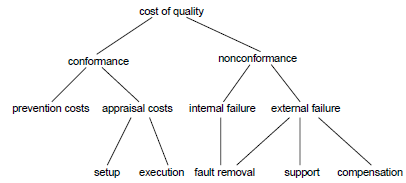
\includegraphics{tipos-custo-arvore.png}
	\label{fig:tipos-custo-arvore}
  \source{\cite{wagner2005}}
\end{figure}

Os custos de \textit{conformance} caracterizam os valores com o intuito de atingir maior qualidade de produto, este por sua vez é divido em custo de prevenção e custo de avaliação. \cite{ wagner2005}

Custos de prevenção são aqueles associados com o intuito de prevenir defeitos antes que possam ocorrer, geralmente são compreendidos por treinamentos, equipamentos, , revisões técnicas formais, atividades de planejamento de qualidade e reviews de produto \cite{wagner2005} \cite{pressman2009engenharia}.

Custos de avaliação compreendem custos relacionados a medidas e extração de métricas, avaliação e auditoria de produtos.\cite{wagner2005}, incluem atividades para ganhar conhecimento da condição do software em análise para cada início de ciclo, incluem: avaliações de processo e entre processos e manutenção \cite{pressman2009engenharia}.

Custos de não conformidade são os custos relacionados aos cenários em que não seguem o planejado e defeitos produzindo um erro e por fim levando à falha \cite{wagner2005}, nesta categoria estão as subcategorias de custos de falha externa e custos de falha interna \cite{pressman2009engenharia}. 

Os Custos de falha externa caracterizam os custos associados aos defeitos após liberação do produto de software para uso, são exemplos: Resolução de chamados, retorno e substituição de produtos e garantias \cite{pressman2009engenharia} enquanto os custos de falha interna são os custos aplicados para remoção de falhas antes de liberação para uso.

O processo de desenvolvimento de um software flui entre os diversos ciclos, e por consequência, diferentes tipos de investimentos são feitos com o intuito de garantiar mainores níveis de qualidade, porém \cite{pressman2009engenharia} afirma que o custo relativo para encontrar e reparar um defeito aumenta consideravelmente na linha do tempo entre as fases iniciais e finais do ciclo de desenvolvimento, sendo assim, custos do tipo \textit{nonconformance} se tornam mais caros ao longo do tempo de projeto, como demonstrado a seguir:

\begin{figure}[H]% H manda colocar exatamente nessa posição no texto (relativa aos parágrafos anterior e posterior)
	\centering
 	  \caption{Crescimento dos custos do tipo \textit{nonconformance} ao longo do tempo de projeto}
		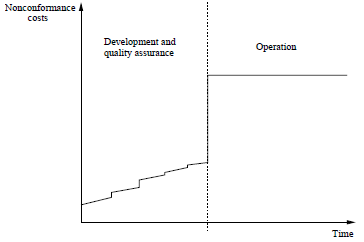
\includegraphics{nonconformance-costs-timeline.png}
	\label{fig:framework-teste}
  \source{\cite{wagner2005}}
\end{figure}




\chapter{Geração automática de dados de teste}

\section{\textit{Symbolic Execution}}
A execução simbólica (\textit{Symbolic Execution}) é um tipo de técnica estrutural para geração de dados de teste que trabalha com base na análise de fluxo de um software para então automaticamente gerar dados de teste \cite{Anand2013}, o ponto diferencial da \textit{Symbolic Execution} para outras técnicas de geração automática de dados de teste é utilizar valores simbólicos ao invés de valores concretos \cite{King1976} nas entradas do software em análise para que estas possam percorrer seu do fluxo de software e asserções lógicas com a finalidade de geração dos conjuntos de dados de entrada.
Valores simbólicos são representações dos valores concretos de variáveis através de expressões simbólicas \cite{Anand2013}
	 

Porém a técnica possui alguns problemas fundamentais as quais limitam sua efetividade em casos práticos de desenvolvimento.

Em qualquer passo de execução simbólica, o estado de execução é formado pelos seguintes atributos: \textit{Symbolic Values}, \textit{Path Constraint} e  \textit{Program Counter}; \textit{Symbolic Values} representam os valores simbólicos e possíveis de serem atribuídos no passo de execução, o \textit{Path Constraint} é uma relação matemática booleana a qual é o resultado da composição de todas as restrições de entradas dos valores percorridos afim de atingir o determinado passo em análise do software;  \textit{Program Counter} é o contador do programa e sempre será responsável por identificar qual será a próxima execução .

A cada passo de análise, o \textit{Path Constraint} é atualizado de maneira que se o seu valor booleano tornar-se infatisfatório, automaticamente o software em análise possui um caminho inatingível, o que torna o fim da análise já que a \textit{Symbolic Execution} não possui caminho para continuar.
Se o caminho em análise possuir um \textit{Path Constraint} satisfatório, quaisquer valores que satisfaçam a condição para que o \textit{Path Constraint} são conjuntos possíveis de dados que podem ser utilizados como entrada para validação e atingir o passo em questão.

Uma \textit{Symbolic Execution Tree} é uma representação compacta de todos os possíveis caminhos descobertos por uma análise simbólica durante a execução simbólica de um programa.

Na \textit{Symbolic Execution Tree} os nós representam os estados do software com seus respectivos \textit{Program Counters}, enquanto as arestas representam as transições entre estes estados

Apesar de ser de execução simbólica ser concebida nos anos 70 por \cite{King1976}, a técnica tem recebido muita atenção nos últimos anos por dois motivos específicos: 
Durante a última década, diversas ferramentas de \textit{Constraint solvers} foram desenvolvidos e o uso destes tornou possível a utilização de  \textit{Symbolic Execution} em um conjunto mais amplo de softwares.

Um outro ponto é que a \textit{Symbolic Execution} possui um consumo computacional muito maior que todas as outras análises, e por conta das limitações computacionais do \textit{hardware} disponível nos anos 80, ela tornou-se inviável em diversos contextos. Porém no contexto atual, o poder computacional é consideravelmente maior do que o hardware da época, o que atraiu diversos pesquisadores para a utilização desta técnica através de \textit{hardwares} mais poderosos.

Porém a \textit{Symbolic Execution} ainda é uma técnica limita por três problemas distintos: \textit{Path explosion}, \textit{Path divergence} e \textit{Complex constrains}. 

\subsection{Funcionamento do Algoritmo de \textit{Symbolic Execution}}

\begin{algorithm}[htbp]
\caption{Exemplo de algoritmo demonstrado por King}
\label{alg:algoritmo-exemplo1}
\begin{algorithmic}[1]
\Procedure{Procedure SUM}{}
\State $SUM: PROCEDURE (A,B,C); $
\State $	X = A + B; $
\State $	Y = B + C; $
\State $	Z = X + Y - B$
\State $	RETURN(Z);$
\State $END$
\EndProcedure
\end{algorithmic}
\source{James C. King, 1976}
\end{algorithm}

\subsection{\textit{Path explosion}}
É difícil de executar simbolicamente todos os subconjuntos de caminhos de uma \textit{Symbolic Execution Tree} pela ação conjunta de dois fatores: Muitos dos softwares de mercado possuem subconjuntos muito grandes de caminhos a serem testados e a execução simbólica de cada software pode demandar em um uso computacional além do disponível. Sendo assim, somente um subconjunto limitado de caminhos, muitas vezes um subconjunto não representativo para o teste por completo, pode ser aplicado para execução.
Este é um problema com um grau alto de complexidade e necessidade de resolução visto que a razão do número de caminhos inatingíveis em relação aos caminhos atingíveis é alta. 

\subsection{\textit{Path divergence}}
Softwares construídos no mundo real possuem diversas implementações em diferentes linguagens, por fim compiladas em um único binário, nestes casos, calcular precisamente as condições requisitam um enorme esforço de desenvolvimento e arquiteturais. Estes casos resultam em divergência de caminhos, ou seja, o caminho que a análise simbólica percorre pode divergir do caminho onde os testes são gerados \cite{Anand2013}. Isto é dado pelo fato de que cada linguagem possui sua própria semântica de descrição que descrevem como os objetos que representam dados possam ser representados \cite{King1976}.

Por conta deste problema, uma execução simbólica de um sistema pode falhar em descobrir um número considerável de caminhos intatingíveis, ou se demandar os modelos pelo usuário, deixar de ser um processo completamente automático.

\subsection{\textit{Complex constrains}}
Resolver todos os \textit{path constraint} pode não ser possível ou trivial, nestes casos o analisador simbólico não consiga resolver conjuntos de \textit{path constraint} que se tornem muito complexos, \cite{Anand2013} afirma que isso é pelo fato de \textit{path constraint} possuírem operações lineares como multiplicações, divisões e funções matemáticas como seno e log que se tornam muito complexas para os atuais \textit{Constraint solvers} disponíveis. Por fim, a habilidade de resolver os caminhos diminui e afeta o resultado final.


Estes três problemas devem ser solucionados para que a técnica possa ser usada amplamente em casos de geração de dados de teste e projetos de desenvolvimento reais.

Apesar de de possuir problemas ainda não resolvidos, a técnica de \textit{Symbolic Execution} vem sendo muito usada para geração de dados de teste, porém seu maior uso atualmente é gerar dados de teste para avaliar cobertura de código e expor possíveis falhas nestes.

A técnica de \textit{Symbolic Execution} pode ser efetivamente utilizada em projetos reais desde que estes possuam duas características: eficiência e automação.

Inicialmente a maioria das aplicações atuais utilizam desta técnica para descobrir possíveis caminhos inatingíveis na \textit{Symbolic Execution Tree} e consequentemente, possíveis instruções que nunca serão executadas e por fim, o esforço manual para aplicação da \textit{Symbolic Execution} deve ser aceitável pelo usuário.

A técnica de \textit{Symbolic Execution} difere de outras técnicas por usar valores simbólicos no lugar de valores concretos em variáveis, porém pode ser usada em combinação com outras técnicas de geração.





Symbolic execution tree
A \textit{Symbolic Execution Tree} caracteriza os caminhos de execução encontrados durante uma execução simbólica.


\section{\textit{Model-Based Testing}}
O \textit{Model-Based Testing}(MBT) é um método formal que utiliza como insumo para geração de dados de teste. os modelos apresentados no software em análise.
Diferente de outras técnicas que procuram fazer a verificação contra modelos formais, o MBT procura reunir conhecimento da corretitude de um software através de abordagens de teste incompletas.

É possível identificar três linhas primárias de estudo em MBT:

\begin{itemize}
	\item \textit{Axiomatic approaches} (AP);
	\item \textit{Finite state machines} (FSM);
	\item \textit{Labeled transition systems} (LTS).
\end{itemize}

\subsection{\textit{Axiomatic approaches}}
As \textit{Axiomatic approaches} de MBT são bases lógicas para cálculo

\subsection{\textit{Finite state machines}}
A abordagem FSM aplicada em MBT inicialmente foi aplicada para resolver problemas funcionais ocorridos em testes de circuitos de hardware, esta foi depois adaptada para trabalhar com protocolos de comunicação.
Na FSM o modelo é formalizado por um tipo específico de máquina de estados chamado \textit{Mealy machine} onde as entradas e saídas formam tuplas em cada transição. A seleção de testes ocorre pela derivação da sequência de nós percorridos de acordo com o critério de cobertura. A maioria das estratégias de FSM trabalham somente com máquinas de estado determinísticas que é considerada uma restrição já que esta limita trabalhar com casos onde os sistemas são reativos ou pouco especificados.

A seleção de testes em FSM é um assunto vastamente pesquisado nos últimos tempos.

Diversas ferramentas de MBT baseadas em FSM não atingem a completamente a cobertura dos testes, eles utilizam critérios de cobertura como cobertura de transições, cobertura de estados e caminhos.

FSM nãp são expressivas o suficiente para representar modelos reais de software.

\section{\textit{Combinatorial texting}}

\textit{Combinatorial Texting} tornou-se uma ferramenta muito utilizada pelo profissionais de garantia de qualidade, nesta o foco é selecionar uma amostra das entradas que seja capaz de cobrir primariamente um subconjunto das combinações dos elementos a serem testados.

A representação mais comum destas é a \textit{combinatorial interaction testing} (CIT) onde as N possíveis combinações de valores dos parâmetros estão contidas nas amostras.

Através dos diversos estágios de teste, profissionais de garantia de gualidade confiaram em heurísticas que aproximassem a cobertura dos dados de entrada e saída, a técnica de \textit{Combinatorial Texting} surgiu com base nos conceitos desta época, nesta, os parâmetros e entradas são configurados como fatores e valores, ou seja, para cada fator $f(i)$, é definido um conjunto de $N$ valores, {${x1, x2,\cdots xn}$}. Deste modelo, os casos de teste são gerados a partir do produto cartesiano dos valores de todos os fatores, esta seleção é feita com base em critérios de cobertura.

Um SUT com cinco fatores, sendo que cada fator possua três valores possui $3^{5}$ ou $243$ configurações possíveis no total.

CIT se tornou tradicionalmente usada baseada em especificações como uma técnica sistemática para aumentar a performance de outros tipos de teste.

Seu foco é detectar um tipo específico de  falha, isso é dado por conta das iterações em cima das combinações das entradas ou das configurações.


\section{\textit{Adaptive random testing}}
A técnica de \textit{Random testing} (RT) é uma das mais populares e fundamentais visto que seu conceito é simples de ser compreendido e implementado. 

A TR é a única técnica de geração de dados de teste onde a habilidade de detecção de falhas pode ser analisada teoricamente.

A \textit{Adaptive random testing} (ART) surgiu como uma evolução da RT

Estudos impíricos demonstram que entradas responsáveis por ocorrência de falhas tendem a formar continuas regiões de falhas enquanto entradas não responsáveis por ocorrência de falhas tendem a formar continuas regiões com ausência de falhas

Neste caso, se conjuntos de dados de teste já utilizados não são capazes de revelar uma falha, novos conjuntos de dados de teste devem explorar regiões diferentes dos conjuntos já utilizados.

Por consequência, conjuntos de dados de teste devem ser capazes de explorar proporcionalmente o domínio de valores possíveis de entrada.

O conceito de de explorar proporcionalmente os diferentes subconjuntos de de domínio de entrada é a base intuitiva de formação do ART

Uma contraproposta ao ART surgiu em 1995, o \textit{Anti-random testing}\cite{malaiya1995}, com o mesmo intuito de explorar proporcionalmente os diferentes subconjuntos de de domínio de entrada, porém com uma diferença fundamental: trata-se de um método determinístico, com a exceção do seu primeiro conjunto de dados gerado ser randômico. A essência do ART é ser um método não determinístico, diferindo também \textit{Anti-random testing} em configurações, já que este possui a restrição de começar a geração com um número de casos de teste já gerados pelo profissional de g	arantia de qualidade.

O ART possui alguns conceitos que necessitam ser elicitados para sua compreensão:

\begin{itemize}
	\item \textit{Failure rate}: Caracterizada por um valor numérico que é a relação do número de entradas causadoras de falhas pela quantidade de valores possíveis no domínio de entrada;
	\item \textit{Failure patterns}: Representa as distribuições e geometria das entradas causadores de falhas;
	\item \textit{Efficiency}: O tempo computacional total requerido, onde um valor menor representa uma eficiência maior  ;
	\item \textit{Effectiveness}: Refere à capacidade de detectar uma falha a qual pode ser medida a partir de métricas de efetividade como P-measure, E-measure, F-measure e etc; A F-measure é uma métrica que demonstra o número de casos de teste necessários para encontrar a primeira falha; A P-measure é a probabilidade de detectar ao menos uma falha e por fim, a E-measure é o número da falhas esperado.
\end{itemize}

Diversas abordagens foram propostas para o conceito de explorar proporcionalmente o domínio de valores possíveis de entrada, e como consequência destas abordagens, diversos algoritmos de ART foram propostos.

\subsection{\textit{Selection of the best candidate}}
O conceito desta abordagem é selecionar o melhor candidato como um próximo conjunto de candidatos, sendo assim, diversos conjuntos de entradas são gerados como candidatos e os melhores candidatos passam por um filtro de restrições onde será escolhido o próximo conjunto.

\subsection{\textit{Exclusion}}
A cada iteração da geração, é definida uma zona de exclusão a partir de casos de teste já executados, os próximos candidatos gerados são gerados fora desta zona afim de gerar uma exploração proporcional.

\subsection{\textit{Partitioning}}
A abordagem \textit{partitioning} utiliza informações das localizações já executadas de casos de teste anteriores, um pouco similar a técnica de \textit{exclusion}, com a finalidade de dividir os domínios de entrada em partições e assim definir à qual partição os próximos casos de teste gerados pertencem.

\subsection{\textit{Test profiles}}

\subsection{\textit{Metric-driven}}


\chapter{Métricas de Software orientados a objeto}

Projeto e desenvolvimento de softwares orientados a objeto são conceitos populares no cenário atual de desenvolvimento de software \cite{srivastava2013}, neste contexto é notável que classes e métodos são estruturas básicas neste gênero de software \cite{kan95}. O desenvolvimento de software orientado a objetos difere de outros paradigmas pois requer uma abordagem voltada para regras de negócio completamente diferente das tradicionais, dado na maneira como a decomposição funcional e fluxo de dados ocorrem  \cite{srivastava2013}.

A análise e projeto de softwares orientados a objeto focam nos objetos como estruturas primárias de computação \cite{kan95} \cite{srivastava2013}, nesta cada classe é composta por dados e operações realizadas, os quais  são representações de uma única entidade real de negócio \cite{srivastava2013}.

As operações realizadas são caracterizadas pelos métodos das classes, a quantidade de funcionalidade, representada por método, agregada ao um software orientado a objeto pode ser estimada com base na quantidade de classe, métodos e variantes destes, utilizados \cite{kan95}. Desta maneira, é comum relacionar métricas de softwares orientados a objeto a valores baseados em atributos de classes e métodos, sejam linhas de código, complexidade, entre outros \cite{kan95}.

As métricas de software tornaram-se elementos primordiais em diversos domínios de Engenharia de software, e principalmente no âmbito de garantia de qualidade, já que toda a informação reúnida por métricas pode ser submetida à diversos tipos de análise e comparação com dados históricos com o objetivo de avaliar e garantir qualidade de software \cite{srivastava2013}. Métricas de software podem ser utilizadas para predizer atributos de qualidade em tempo de execução, inclusive para aplicações cujo requisito é ser uma aplicação de tempo real \cite{srivastava2013}. O real valor de métricas de software vem da sua representação dos atributos de software externos, muitos destes com alto valor de negócio, como confiabilidade, mantenibilidade, reusabilidade, testabilidade e eficiência \cite{srivastava2013}, os quais são requisitos de qualidade descritos pela ISO9126 \cite{Zeiss2007}.



%Um grande número de métricas foi proposto ao longo do tempo pela literatura \cite{srivastava2013}.



\section{Medidas diretas}
Uma medida direta de software é uma métrica a qual o cálculo de seu valor não depende nenhum outro atributo além do principal utilizado em seu cálculo \cite{srivastava2013}. Exemplos claros de medidas em produtos são: LOC (\textit{Lines of code}), velocidade de execução, tamanho de memória, quantidade de defeitos reportados \cite{srivastava2013}.


\section{Medidas indiretas}
Uma medida indireta de software é uma métrica a qual envolve a medida de um ou mais atributos de software\cite{srivastava2013}. As medidas diretas são, em geral, mais fáceis de serem coletadas.


\section{O conjunto de métricas CK}

Em 1994 Chidamber e Kemerer proporam seis métricas de projeto e complexidade de softwares orientados a objeto, as quais, futuramente, tornaram-se o conjunto de métricas CK \cite{kan95}. 

Chidamber e Kemerer aplicaram as seis métricas do conjunto (as quais serão definidas em seções posteriores) em estudos empíricos de duas empresas, uma usando C++ e outra Smalltalk \cite{kan95}, o sumário desta é demonstrado na tabela.

\subsection{\textit{Weighted methods per class (WMC)}}
A WMC é uma métrica contabilizada pela soma das complexidades dos métodos, onde a complexidade é dada pelo \textit{cyclomatic complexity number}  de McCabe (CCN)\cite{kan95} \cite{watson96}. Medir o \textit{cyclomatic complexity number} não é trivial de implementação dado que nem todos os métodos são acessíveis de acordo com a hierarquia dos objetos, isso é resultado por conta da herança aplicada no projeto do componente \cite{kan95}.

\subsection{\textit{Depth of inheritance tree (DIT)}}
A DIT é uma medida que compreende o valor do comprimento máximo de um caminho em uma árvore de herança, este comprimento é dado pela distância entre o nó em análise até o nó raíz \cite{kan95}. A definição da DIT baseia-se na premissa de que desenvolvedores lidam com linguagens de programação orientadas a objeto as quais permitam que uma classe possua no máximo uma classe pai \cite{bruntink04}, linguagens alheias a este conceito são conhecidas por possuir herança múltipla, presente em linguagens como C++ e Python. Muitas linguagens orientadas a objeto não suportam herança múltipla por conta do problema do diamante, supondo a estrutura a seguir:

\begin{figure}[H]% H manda colocar exatamente nessa posição no texto (relativa aos parágrafos anterior e posterior)
	\centering
 	  \caption{Exemplo de problema do diamante}
		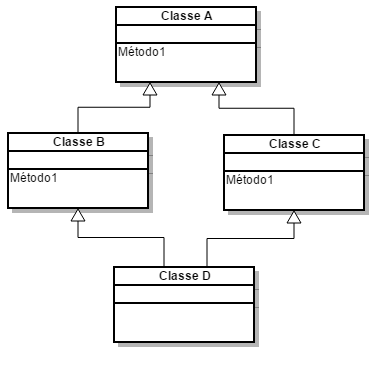
\includegraphics{diagrama_diamante.png}
	\label{fig:tipos-custo-arvore}
  \source{Gustavo Ramos, 2017}
\end{figure}

Neste caso, um objeto instanciado do tipo D possui acesso para executar o \textbf{Método 1}, porém o compilador pode não saber a qual referência de \textbf{Método 1} executar já que o objeto do tipo D herda tanto de B e de C quanto de A, todos os quais possuem o \textbf{Método 1}. Este caso é conhecido por problema do diamante, por conta deste, linguagens como Java não permitem a herança múltipla.Dada a premissa de que a linguagem do software em análise não suporta herança múltipla, ao calcular o DIT, o número de ancestrais do nó $c$ em análise, corresponde à profundidade de $c$ na árvore de herança \cite{bruntink04}. A fórmula que descreve o cálculo da DIT para um determinado nó $c$ é dado a seguir:

\begin{equation}
  DIT(c) = |Ancestrais(c)|
	\label{eq:calc-dit}
\end{equation}

\subsection{\textit{Number of children of a class (NOC)}}

O NOC é uma métrica de simples cálculo, caracterizada pelo número de sucessores imediatos(subclasses) na árvore de hierarquia, calculada com base em  uma classe $c$ em análise \cite{kan95}. Seu cálculo é dado pela fórmula a seguir:

\begin{equation}
  NOC(c) = |Filhos(c)|
	\label{eq:calc-noc}
\end{equation}


\subsection{\textit{Coupling between object classes (CBO)}}
Uma classe $A$ é acoplada a uma classe $B$ se a classe $A$ invoca uma método ou utiliza uma variável de uma instância de $B$ \cite{kan95}, sendo assim, o CBO é dado pelo número de classes a qual uma classe $c$ em análise está acoplada, ou seja, seu cálculo é dado por:

\begin{equation}
  CBO(c) = |Quantidade de classes que relaciona(c)|
	\label{eq:calc-cbo}
\end{equation}

\subsection{\textit{Response for a class (RFC)}}
O RFC é caracterizado pelo número de métodos que podem ser executados na resposta de uma mensagem recebida por uma instância de uma classe \cite{kan95}, ou seja, o RFC é uma contagem do número de métodos de uma classe $c$ em análise e o número de métodos de outras classes que são invocados pelos métodos de $c$ \cite{bruntink04}.

Quanto maior o número de métodos que podem ser invocados indiretamente através de uma chamada de um método, maior a complexidade de uma classe, basicamente o RFC captura o tamanho de conjunto de respostas de uma classe \cite{kan95}. O RFC é calculado pelo número de métodos locais mais o número de métodos chamados por métodos locais \cite{kan95}.


\subsection{\textit{Lack Of Cohesion Of Methods (LCOM)}}
A independência pode ser medida por critérios qualitativos: coesão e acoplamento, a coesão é a medida relação funcional de um módulo \cite{pressman2009engenharia}, neste contexto, a coesão de uma classe é dada pela proximidade de métodos locais à instâncias de variáveis na classe, alta coesão indica uma boa subdivisão das classes \cite{kan95}.

A métrica LCOM representa a dissimilaridade dos métodos em uma classe pelo uso de instâncis de variáveis, a alta de coesão aumenta a complexidade e por consequência, oportunidade de ocorrência de erros durante o processo de desenvolvimento \cite{kan95}.

\section{Métricas de Lorenz e regras de ouro}






Baseado nestes conceitos, lorenz(1993) propôs 11 métricas de projetos de softwares orientados a

objeto e diretivas sobre os valores destas

Enquanto a maioria destas métricas são relacionadas à design de código e implementação, as

métricas Agerage number of comment Lines, Number of problem reports per class e numbers od

classes and methods thrown aray se destacam por terem propósitos diferentes.

A tabela proposta por lorenza é definida a seguir:


\section{Modelo proposto por Srivastava e Kumar}

Srivastava e Kumar proporam em 2013 um modelo de métricas para validação de qualidade de software com a justificativa de que nenhuma das métricas tratavam acoplamento ou similaridades como relações transacionais, sendo assim, métricas que mapeiam estas características são passíveis de incorporação no modelo. No estudo em questão, diversos dados foram coletados de projetos orientados a objeto nas linguagens Java e C++ e neste constatado que diversas métricas são baseadas em ideias similares e representam informações redundantes, sendo assim, foi validado que um subconjunto de métricas pode ser utilizado para predição de falhas.

O modelo proposto por \cite{srivastava2013} atingiu um nível de acurácia superior a 80\% na predição de falhas em classes.

\begin{figure}[H]% H manda colocar exatamente nessa posição no texto (relativa aos parágrafos anterior e posterior)
	\centering
 	  \caption{Modelo de qualidade proposto por Srivastava e Kumar}
		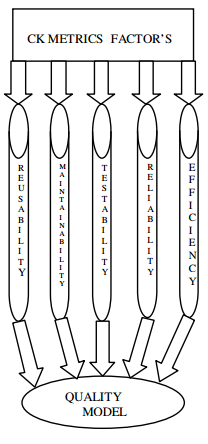
\includegraphics{modelo_srivastava_kumar.png}
	\label{fig:tipos-custo-arvore}
  \source{\cite{srivastava2013}}
\end{figure}


\chapter{Proposta de projeto}

% ----------------------------------------------------------
% ELEMENTOS PÓS-TEXTUAIS
% ----------------------------------------------------------
\postextual
% ----------------------------------------------------------

% ----------------------------------------------------------
% Referências bibliográficas
% ----------------------------------------------------------
\bibliography{referencias}

% ----------------------------------------------------------
% Glossário
% ----------------------------------------------------------
%
% Consulte o manual da classe abntex2 para orientações sobre o glossário.
%
%\glossary

% ----------------------------------------------------------
% Apêndices
% ----------------------------------------------------------

% ---
% Inicia os apêndices
% ---
\begin{apendicesenv}

% Imprime uma página indicando o início dos apêndices
%\partapendices

%-------------------------------------------------------------------------
% Comentário adicional do PPgSI - Informações sobre ``apêndice''
%
% Para todos os captions/(títulos) (de seções, subseções, tabelas, 
% ilustrações, etc):
%     - em maiúscula apenas a primeira letra da sentença (do título), 
%       exceto nomes próprios, geográficos, institucionais ou Programas ou
%       Projetos ou siglas, os quais podem ter letras em maiúscula também.
%
% Todas  as tabelas, ilustrações (figuras, quadros, gráficos, etc. ), 
% anexos, apêndices devem obrigatoriamente ser citados no texto.
%      - a citação deve vir sempre antes da primeira vez em que a tabela, 
%        ilustração, etc., aparecer pela primeira vez.
%
%-------------------------------------------------------------------------



\end{apendicesenv}

%---------------------------------------------------------------------
% INDICE REMISSIVO
%---------------------------------------------------------------------
%%%%%MF\phantompart
%%%%%MF\printindex
%---------------------------------------------------------------------

\end{document}
